% Walk-forward ladder factor-book analysis (L2 / L4 / L5 / L7).
% Build: tectonic wf_book_analysis.tex   (figures expected in figures/)
\documentclass[11pt,a4paper]{article}

\usepackage[margin=2.6cm]{geometry}
\usepackage{graphicx}
\usepackage{booktabs}
\usepackage{float}
\usepackage{caption}
\usepackage{enumitem}
\usepackage{xcolor}
\usepackage{microtype}
\usepackage{newtxtext,newtxmath}
\usepackage[hidelinks,pdfauthor={Luca Wuerker},
            pdftitle={Factor Books of the Walk-Forward Ablation Ladder}]{hyperref}

\definecolor{grey}{RGB}{96,93,84}
\captionsetup{font=small,labelfont=bf,width=.92\textwidth}
\setlist{itemsep=2pt,topsep=4pt}

\title{\bfseries Factor Books of the Walk-Forward Ablation Ladder}
\author{Luca W\"urker}
\date{August 2026}

\begin{document}
\maketitle

\begin{abstract}
\noindent Factor-level analysis of the alpha books produced by four evolutionary
research runs on the survivorship-bias-free Nasdaq-100 point-in-time panel
(2010--2026): L2 (evolution without retrieval), L4 (knowledge-graph retrieval),
L5 (L4 plus an adversarial hypothesis debate) and L7 (L5 plus cross-run memory).
Each run evolved for twenty generations under a two-phase progressive reveal;
generations 11--20 each first trade one unseen six-month block of 2021--2026
before the population may adapt to it, so the last five years form an honest
walk-forward record. All numbers are signal-level information coefficients (IC);
no position construction or costs enter.
\end{abstract}

\section{Per-factor performance}

\begin{figure}[H]\centering
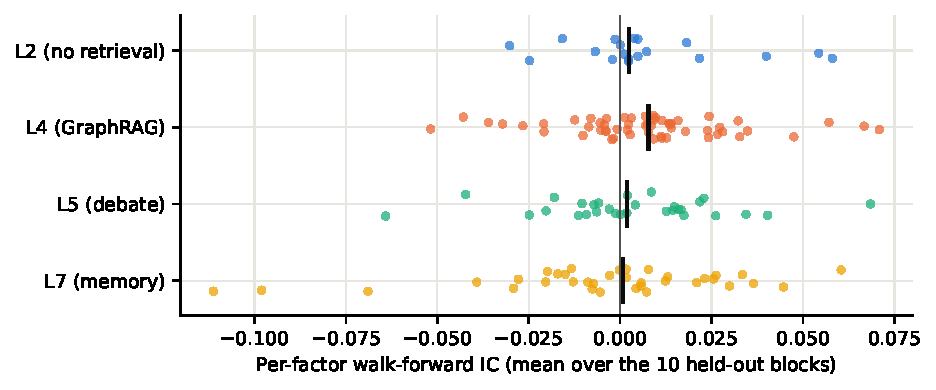
\includegraphics[width=.95\textwidth]{figures/f1_factor_ic_strip}
\caption{Per-factor IC averaged over the ten held-out walk-forward blocks; the
black bar marks the median. L4 produces both the largest book (57 factors) and
the highest median walk-forward IC ($0.008$, 65\% positive); the memory arm L7
has the widest left tail.}
\end{figure}

\begin{figure}[H]\centering
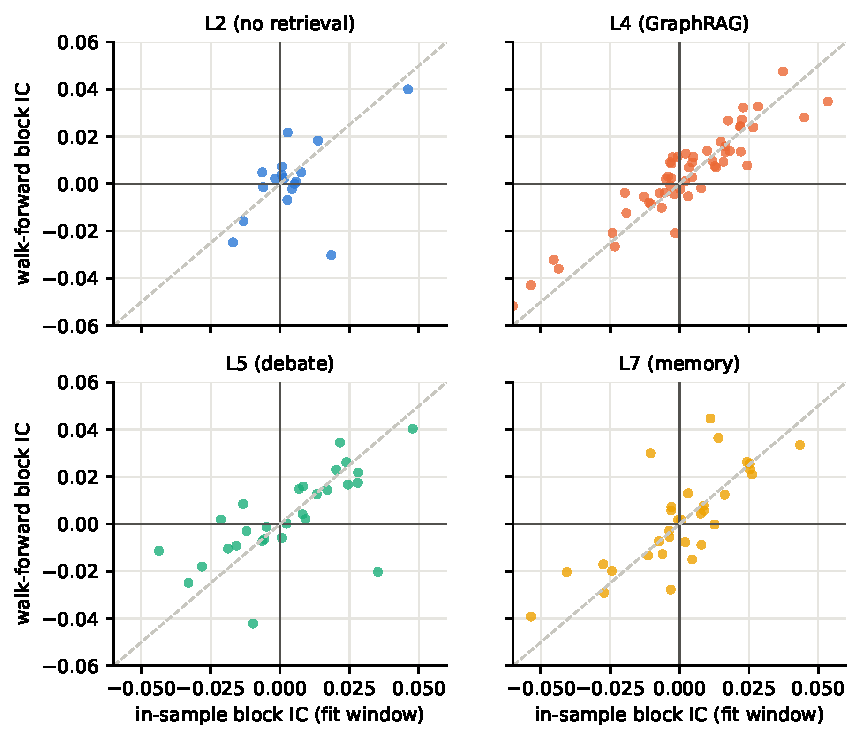
\includegraphics[width=.88\textwidth]{figures/f2_ic_retention}
\caption{In-sample versus walk-forward per-factor IC (block metric on both
sides). Per-factor edge survives out of sample in every arm --- mean $|$IC$|$ is
essentially unchanged from fit window to walk-forward --- and the rank
correlation is high for L2/L4/L7 ($0.83$--$0.94$; L5 $0.24$ due to two
outliers).}
\end{figure}

\section{Combining the book into one signal}

\begin{figure}[H]\centering
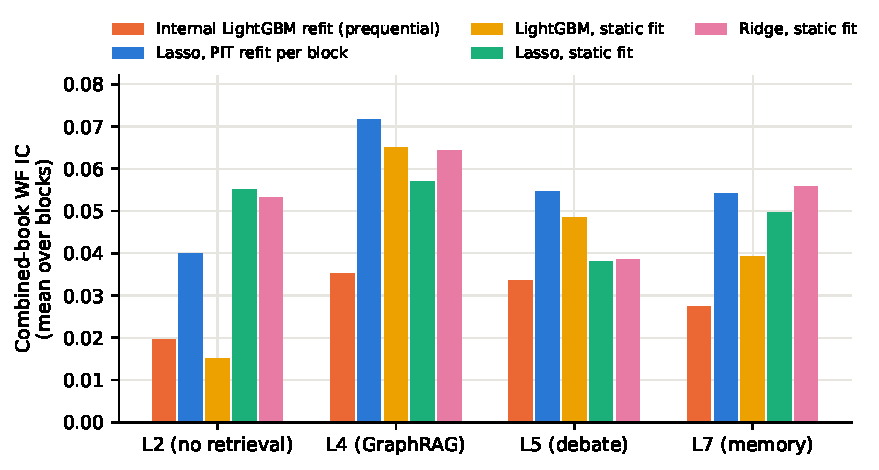
\includegraphics[width=.95\textwidth]{figures/f3_combined_book}
\caption{Combined-book walk-forward IC (mean over the ten blocks) for five
combiners. The run's own prequential LightGBM refit --- the score the evolution
sees internally --- is the \emph{weakest} deployment combiner in every arm; a
point-in-time lasso refit per block or a simple static ridge adds 50--100\%.
L4 leads at every combiner (PIT lasso $0.072$).}
\end{figure}

\begin{figure}[H]\centering
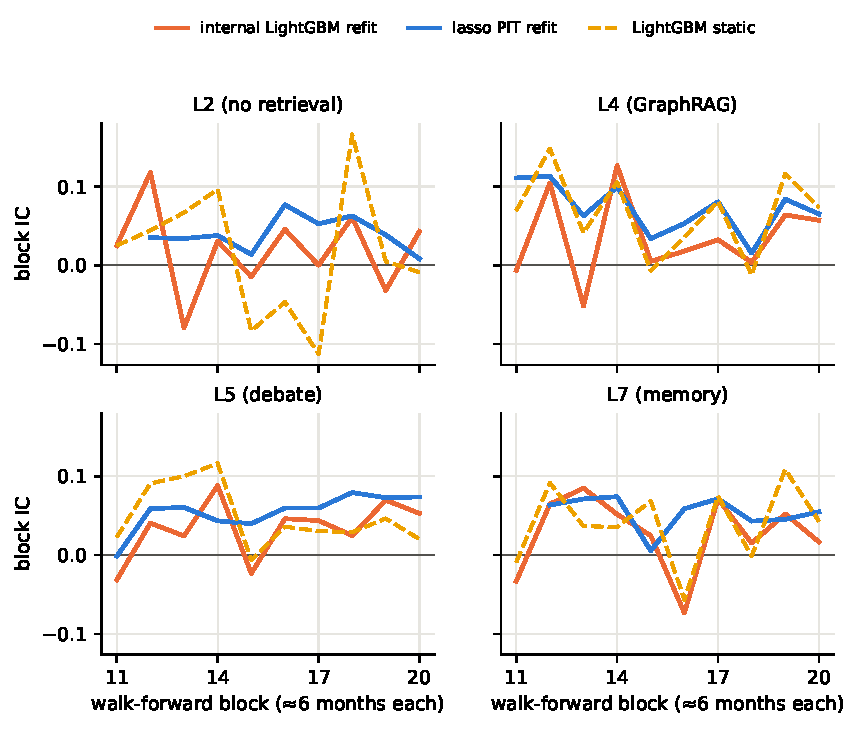
\includegraphics[width=.95\textwidth]{figures/f4_blocks}
\caption{Block-by-block combined IC over the ten held-out blocks (2021--2026).
The PIT lasso is positive in 37 of its 38 valid arm-blocks; the tree-based
combiners are right on average but far noisier.}
\end{figure}

\section{Archive dynamics over the evolution}

\begin{figure}[H]\centering
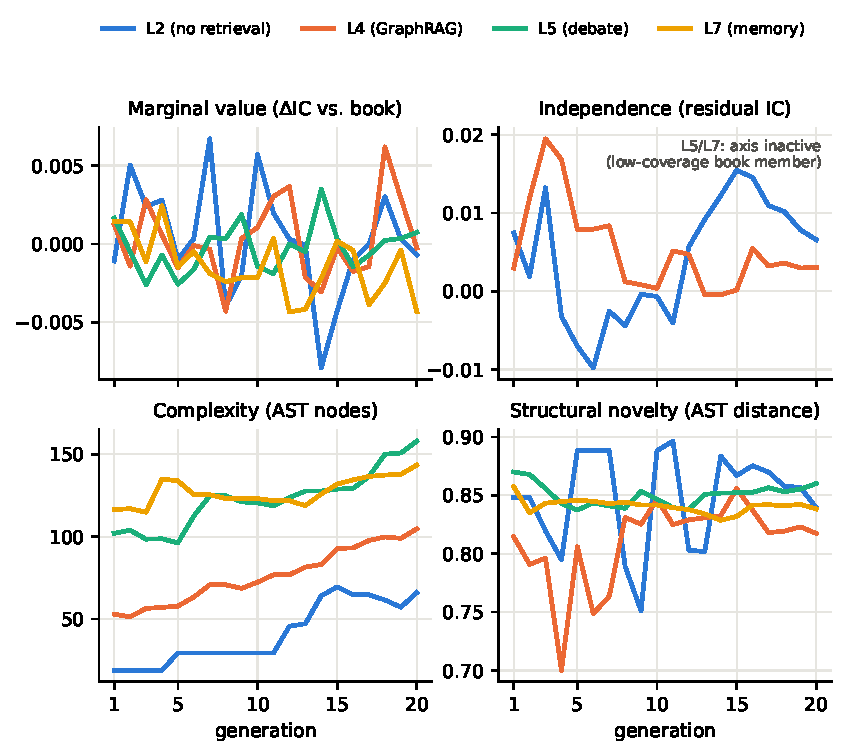
\includegraphics[width=.95\textwidth]{figures/f5_pareto_axes}
\caption{Mean of the four Pareto objectives across the factors that survive into
the final archive, per generation (values carried forward between re-scores).
Marginal value hovers near zero by construction (each survivor is measured
against the rest of the book); complexity ratchets upward in every arm while
structural novelty stays flat around $0.85$ --- the parsimony objective slows
but does not stop code growth. The residual-IC independence objective was
silently inactive in L5/L7: once a factor with sparse coverage enters the book,
the orthogonalisation has too few jointly-complete rows and returns no value.}
\end{figure}

\begin{figure}[H]\centering
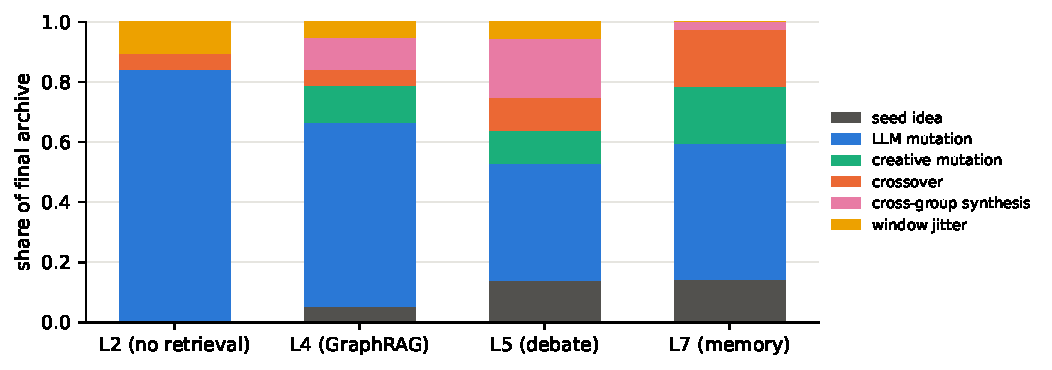
\includegraphics[width=.95\textwidth]{figures/f9_operator_mix}
\caption{Origin of the surviving factors. Direct LLM mutation dominates
everywhere, but the share of survivors from recombination operators (crossover,
cross-group synthesis) grows with the richer configurations, reaching a third
of the book in L5/L7.}
\end{figure}

\section{Diversity and selection}

\begin{figure}[H]\centering
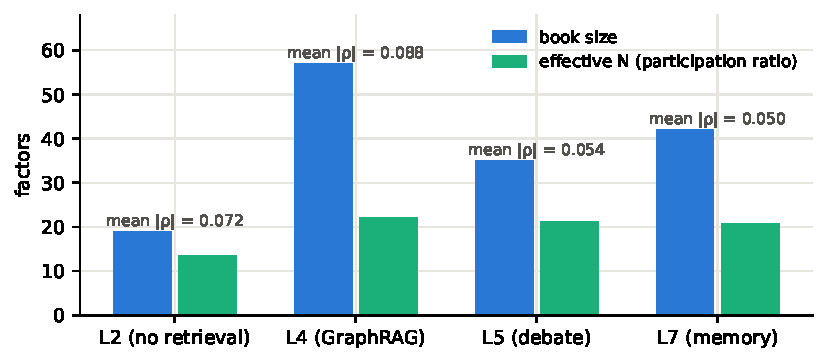
\includegraphics[width=.95\textwidth]{figures/f6_diversity}
\caption{Book diversity via the participation ratio of the signal-correlation
eigenvalues, $N_{\mathrm{eff}}=(\sum_i\lambda_i)^2/\sum_i\lambda_i^2$. All
evolved books are highly diverse (mean $|\rho|\le 0.09$); L4's 57 factors carry
about 22 effective independent bets, and the smaller L5/L7 books reach almost
the same effective dimension with fewer factors.}
\end{figure}

\begin{figure}[H]\centering
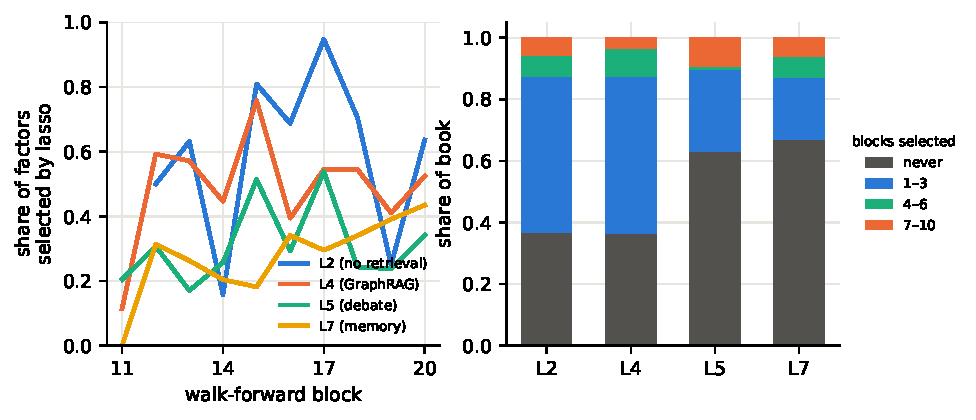
\includegraphics[width=.95\textwidth]{figures/f7_lasso_sparsity}
\caption{Lasso sparsity under the point-in-time protocol (cross-validated
refit before each block). Left: the selected share swings widely between
blocks. Right: over the ten refits, 37\% (L2/L4) to 63--67\% (L5/L7) of
factors are never selected, and fewer than 15\% are selected in most blocks
--- yet the combined IC is stable, indicating substantial interchangeability
within each book.}
\end{figure}

\begin{table}[H]\centering\small
\caption{Cross-validated lasso per phase of the walk-forward period: mean
number of selected factors (of available) and mean block IC.}
\begin{tabular}{lccc}
\toprule
 & 2021--23 & 2023--25 & 2025--26 \\
\midrule
L2 (no retrieval) & 10.5 / 18.5 \hfill (.034) & 12.3 / 18.8 \hfill (.045) & 10.0 / 18.3 \hfill (.036) \\
L4 (GraphRAG)     & 23.7 / 57.0 \hfill (.095) & 33.3 / 62.8 \hfill (.067) & 30.3 / 61.0 \hfill (.055) \\
L5 (debate)       & \phantom{0}9.0 / 39.7 \hfill (.039) & 15.0 / 37.5 \hfill (.051) & 10.7 / 39.0 \hfill (.075) \\
L7 (memory)       & \phantom{0}7.0 / 37.3 \hfill (.067) & 11.0 / 43.3 \hfill (.052) & 18.0 / 46.3 \hfill (.048) \\
\bottomrule
\end{tabular}
\end{table}

\section{Key observations}

\begin{enumerate}
\item \textbf{Factor-level edge transfers; the combiner is the fragile part.}
Mean per-factor $|$IC$|$ is fully retained from the fit window to the 2021--2026
walk-forward in all four arms, while the combined-model IC depends strongly on
the combiner class: simple penalised linear models beat the boosted-tree
combiner the search itself uses, in every arm.
\item \textbf{Retrieval grounding (L4) is the strongest single addition.} It
yields the largest book, the best per-factor medians, the highest effective
diversity, and the best combined walk-forward IC at every combiner.
\item \textbf{Debate and memory did not pay for themselves at the book level.}
L5/L7 books are half positive at the factor level and combine to $\sim$0.055
(PIT lasso) versus L4's 0.072, at comparable diversity.
\item \textbf{Selection is unstable, performance is not.} Which factors the
lasso picks changes sharply between refits and a third to two-thirds are never
picked, yet the combined IC stays positive in 37 of 38 valid arm-blocks --- the
books are internally redundant in a useful, robust sense.
\item \textbf{Two mechanical caveats for the write-up.} Complexity drifts
upward over generations despite the parsimony objective; and the residual-IC
independence objective silently deactivates once any sparse-coverage factor
enters the book (L5/L7 effectively evolved on three objectives), which should
be fixed by orthogonalising on pairwise-complete data.
\end{enumerate}

\end{document}
